\subsubsection{Functional Principle} \label{section:license-google-functional}
\begin{itemize}
  \item flow überprüfen...
    \item query trusted server
    \item manually implemented by developer, code is provided
    \item simple checking and callback with google
    \item library manages all, sends request to server, drm, does not interfer with app logic
    \item developer handles result while library handles rest, full control of what happens with callback
    \item additional information send, licensechecker gets packagename, nonce, callback
    \item play service adds google account
    \item server checks whether purchased and responds
    \item security is important, public/private key encryption provided by google, tampering protection
    \item requires online connection, google play services at first time
    \item when how often done by developer
    \item replaces old copy protection
\end{itemize}
\begin{figure}[h]
    \centering
    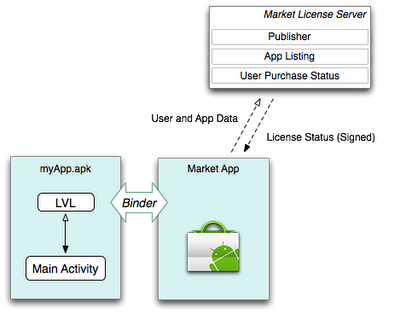
\includegraphics[width=0.8\textwidth]{data/lvl.png}
    \caption{Google's implementation of license checking \cite{developersLicensingOverview}}
    \label{fig:lvl}
\end{figure}
